 \documentclass{standalone}
 \usepackage{tikz}
\usepackage{tkz-graph}
 \begin{document}

\begin{tikzpicture}
  \SetGraphUnit{5}
    \tikzset{
  EdgeStyle/.append style = {->} }
   \tikzstyle{VertexStyle}=[shape = circle, draw, minimum size = 30pt]
 

  \node (s2) at (0,1.5) {
\includegraphics[width = 1cm]{rrh.png}};
  \node (s1) at (0,0) {
\includegraphics[width = 1cm]{rrh.png}};
  

   \node (b1) at (10,0.75) {
\includegraphics[width = 1cm]{bbu.png}};

 
  
   \node (t1) at (4,0.75) {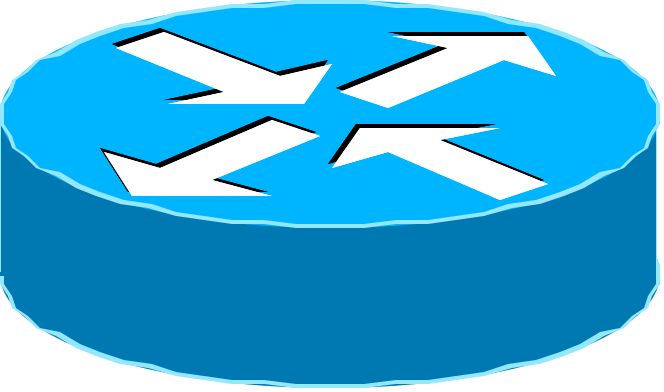
\includegraphics[width = 1cm]{switch.png}};
    \node (t2) at (6,0.75) {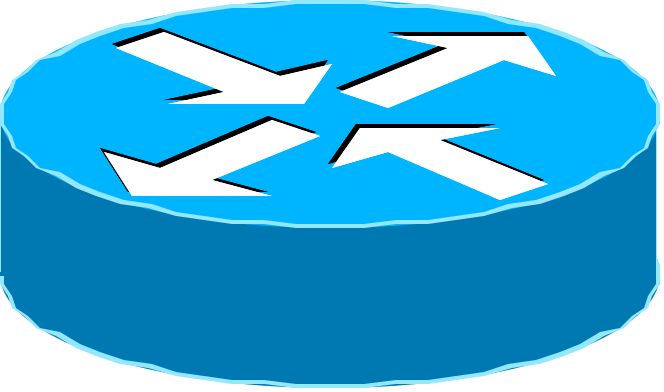
\includegraphics[width = 1cm]{switch.png}};
  \node (t3) at (8,0.75) {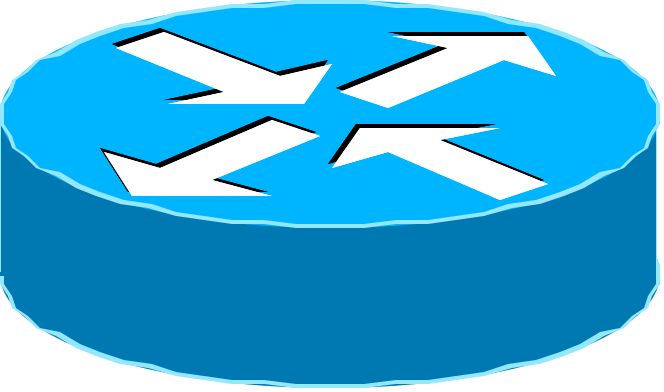
\includegraphics[width = 1cm]{switch.png}};
 \node (t4) at (7,2.25) {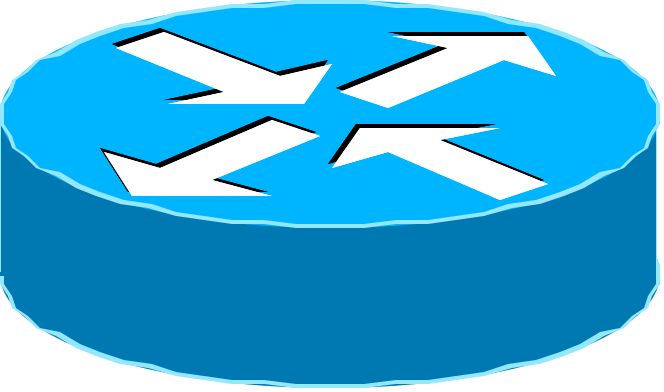
\includegraphics[width = 1cm]{switch.png}};

 \path (s1) [->,blue,thick] edge (t1);
 \path (s2) [->,green,thick] edge (t1);


 \path ([yshift=-0.5mm]t1.east) [->,blue,thick] edge ([yshift=-0.5mm]t2.west);
 \path (t1.east)  [->,green,thick] edge  (t2.west);
 \path (t2) [->,blue,thick] edge (t3);
 \path (t2) [->,green,thick] edge (t4);
 \path (t4) [->,green,thick] edge (t3);
 \path ([yshift=-0.5mm]t3.east) [->,blue,thick] edge ([yshift=-0.5mm]b1.west);
 \path (t3.east)  [->,green,thick] edge  (b1.west);



\end{tikzpicture}
 \end{document}